\chapter{ Problem definition, Initial Design using Design Thinking approach, Experimentation / Design calculations / Flowcharts / Algorithms }
\section{Problem definition}
Systems analysis is a problem solving technique that decomposes a system into its component pieces 
for the purpose of the studying how well those component parts work and interact to accomplish their purpose~\cite{SystemsAnalysisandDesign}.
\lipsum[1-1]

\section{Initial Design using Design Thinking approach}
\lipsum[2-2]

\section{Experimentation}
\lipsum[3-3]

\section{Design calculations}
\lipsum[4-4]

\section{Flowcharts}
Initialization module takes input from get configuration module and sets properties of CA, and places one CSC in center, 
surrounded by ES with FD as fiber density and about $\sigma$ number of ES (Figure \ref{Initialization} and 
Figure \ref{InitializationFlowChart}).
It then calls simulation module.
  
  \begin{figure}[H]
	  \centering
	  \fbox{ 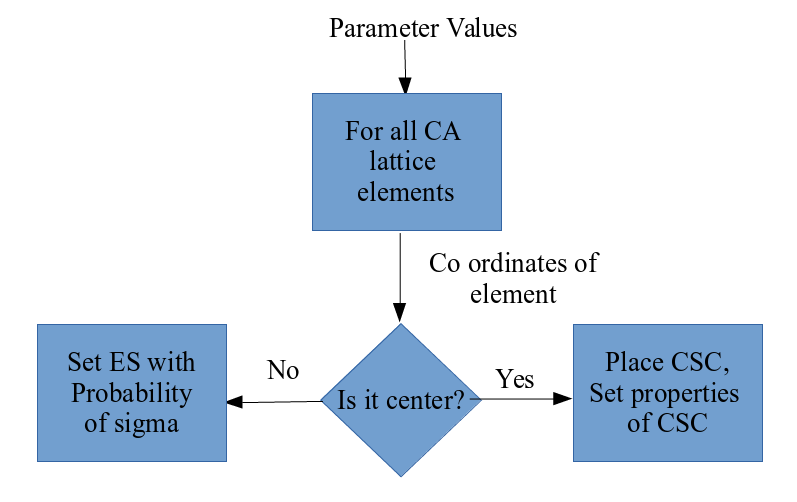
\includegraphics[scale=0.35]{images/InitializationFlowChart.png} }
	  \caption{Flow for initialization of Cellular Automata}	
	  \label{InitializationFlowChart}
  \end{figure}   

  \begin{figure}[H]
	  \centering
	  \fbox{ 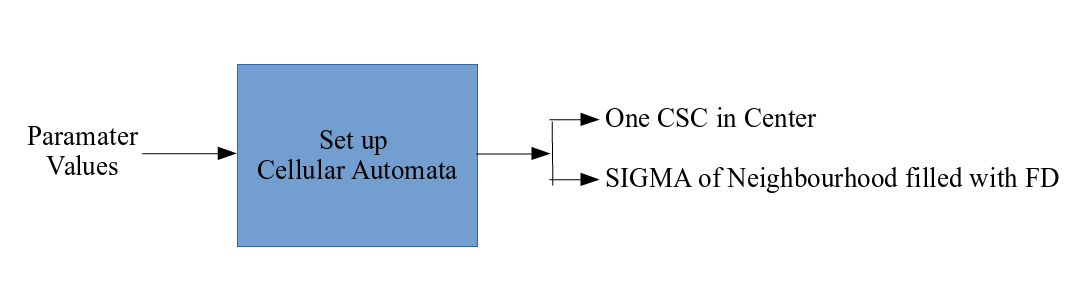
\includegraphics[scale=0.35]{images/Initialization.png} }
	  \caption{Initialization of Cellular Automata}
	  \label{Initialization}
  \end{figure}

\section{Algorithms}

\noindent Algorithm: Cell Division, checks the type of cell and initiate respective divide.\\\

\begin{algorithm}[H]
 %\caption{Cell Division}
     \SetAlgoLined
     \KwData{present cell and neighbourhood ES details}
     \KwResult{ initiate CSC or TAC division if conditions hold }
     
	\begin{algorithmic}
	      \IF{  cell.type == CSC }
		\STATE cell.divideCSC();
		\ELSIF{  cell.type == TAC }
		\STATE cell.divideTAC();
	      \ENDIF
	\end{algorithmic}
		    
\end{algorithm}


\noindent Simulation algorithm: At each iteration of the simulation, 
a CA cells is randomly selected and evolved based on some mechanistic rules (Algorithm of Simulation). 
If the selected site is of type S (free space) or E (ECM site) then nothing happens. 
Else (if selected site is C (cancer cell)) the age of the cell is increased by an amount $\delta$ which is determined based on 
fiber density of the neighbourhood as described in Equation \ref{increaseAgeByDelta} ~\cite{klein2009, ulrich2009}. 
After increasing cell age, the cell select a neighbouring ECM\_SITE or FREE\_SITE randomly. 
\begin{equation}
 \delta =  1 + 1.125 *  \frac{[FD]}{[FD]+1}
 \label{increaseAgeByDelta}
\end{equation}


\noindent BCs can move into or divide in neighbourhood ES only if FD = 0. 
If there is no ECM\_SITE or FREE\_SITE in neighbourhood of cell, 
cell undergo transformation where it can either convert to a TDC. If the type of cell is TAC and its current $\beta$ value is greater than 0, 
or die out and if the type of cell is TDC and its age is equal to $\gamma$ value.\\\

\begin{algorithm}[H]
	\label{algori}
	%\caption{Simulation algorithm}algori
	\SetAlgoLined
	%\KwData{ Cellular Automata }
	%\KwResult{ CSC, TAC division, and proliferation of Biological Cells, Run ITERATIONS times, change in properties of ES and also Type of Biological Cells }
	%Save initial state of system;\\\
	\noindent Algorithm of Simulation\\
	\For {\rm 1 to NUM\_OF\_ITERATIONS}
	{
		\For {\rm ROWS * COLUMNS times }
		{
			cell  $\gets$ Randomly select an automata cell;			
			\eIf{\rm (cell.type == E OR  cell.type == S)}
			{
				// No action is performed
			}
			{   
				// Increase cell age by $\delta$, $\delta =  1 + 1.125 *  \frac{[FD]}{[FD]+1}$; $\delta$ = 1 for TDC; \\
				cell.age  $\gets$ cell.age + $\delta$  \\				
				\eIf{\rm There is no ECM\_SITE or FREE\_SITE in neighbourhood}
				{
					\If{\rm cell.type ==  TAC AND cell.$\beta$ = 0}
					{				      
						cell.type = TDC
					}					
					\If{\rm cell.type ==  TDC AND cell.age = $\gamma$}
					{ 
						cell.type = ECM\_SITE
					}
				}
				{
					neighbourES  $\gets$ randomly select one ECM\_SITE from neighbourhood;										
					\eIf{\rm neighbourES.FiberDensity = 0}
					{				      						
						\eIf{\rm cell.age $\ge$  DOUBLING\_TIME and cell.type == CSC or TAC }
						{
							\eIf{\rm cell.type ==  CSC }
							{				      
								Perform symmetrical division of cell with probability $\alpha$ or asymmetrical division with probability (1-$\alpha$).
							}
							{ 					  
								Generate two daughter cells with $\beta$ less than the mother $cell$.
							}	
						}
						{				    
							Move $cell$ to neighbourES free site with probability $\mu$.   	      
						}						
					}
					{												
						$\lambda = 0.5625\times \frac{{[FD]}}{[FD]+1} $\; 
						neighbourES.FiberDensity = neighbourES.FiberDensity - $\lambda$ ;
					}
				}								
			}	   	   			
		}
		Save state of system;
	}
\end{algorithm}
